\documentclass[12pt]{article}
\usepackage{graphicx}
%\usepackage{comment}
\usepackage{hyperref}
\usepackage{amsmath}
%\usepackage{siunitx}
\usepackage{subcaption}
%\usepackage{amssymb}
\usepackage{float}
\usepackage{wrapfig}
\usepackage{caption}
\usepackage{etoolbox}
\usepackage{enumitem}
\usepackage{verbatim}
%\setlength{\leftmargin}{1}
\usepackage{geometry}
\usepackage{hyperref}
 \geometry{
 left=15mm,
 right=15mm,
 %top=20mm,
 %bottom=20mm,
 }
\makeatletter
\preto{\@verbatim}{\topsep=0pt \partopsep=0pt }
\makeatother
\date{}

\begin{document}
\begin{titlepage}
\begin{center}
\Huge
\textbf{User Guide for \\
AMMCR: Ab-initio model for Mobility and Conductivity Calculation by Using Rode Algorithm\\} 
\vspace{5mm}
\Large 
By: Anup Kumar Mandia, anup12352@gmail.com
\end{center}
\end{titlepage}
  
\tableofcontents

\newpage
  
  
\section{Introduction}
Ab initio model for mobility and conductivity calculation by using the Rode Algorithm (AMMCR) is a module to calculate various transport coefficients at low electric field with inputs calculated from first principles. AMMCR solves the Boltzmann transport equation within Rode's iterative scheme. For more detailed information, see \cite{anup1,anup2,anup3}. It is written in C++. Currently, it is interfaced with the Vienna Ab initio Simulation Package (VASP). It is very simple to use. Once compiled, it produces an executable file called AMMCR. The executable can be run in a directory where four VASP output files, OUTCAR, EIGENVAL, PROCAR, and DOSCAR, are present. \\

\begin{figure}[!t]
	\centering
	{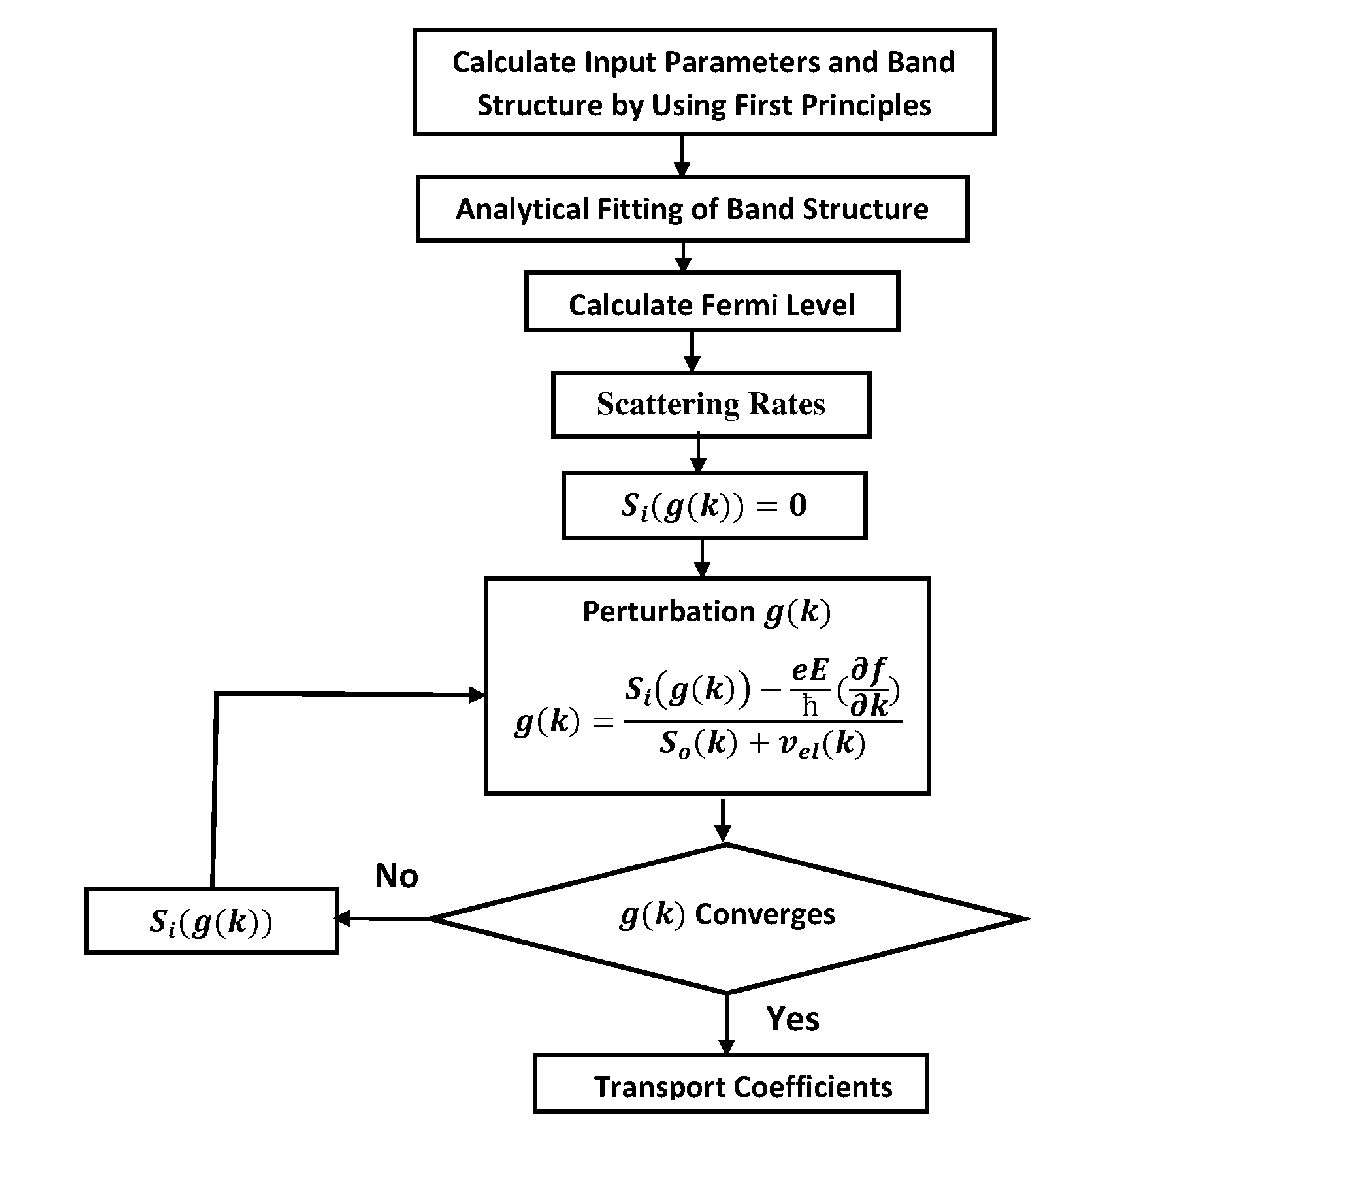
\includegraphics[height=0.85\textwidth,width=0.85\textwidth]{flowchart.pdf}}
	\quad
	\caption{Flowchart for transport coefficient calculation from input calculated from DFT. For more detail, refer to \cite{anup1, anup2, anup3}. }
	\label{flowchart}
\end{figure}

If the band structure calculation is done in spin-polarized mode, the code automatically detects it and produces two sets of results: For majority and minority spin electrons. \\

The specification of the simulation conditions, such as temperature, doping concentration, external electric field, etc., as well as the materials constants, are provided in a file called \textbf{input.dat}. \\

There is also a YouTube video about how to compile and run the AMMCR code: \\ \href{https://youtu.be/II-7I68iPnI}{https://youtu.be/II-7I68iPnI}. \\ 

If you use AMMCR for your research, please cite the following article: \\
\textbf{Anup Kumar Mandia, Bhaskaran Muralidharan, Jung-Hae Choi, Seung-Cheol Lee and Satadeep Bhattacharjee, AMMCR: Ab initio model for mobility and conductivity calculation by using Rode Algorithm, Computer Physics Communications, Volume 259, 2021, 107697, ISSN 0010-4655, \href{https://doi.org/10.1016/j.cpc.2020.107697}{ https://doi.org/10.1016/j.cpc.2020.107697.}} \\ 

\subsection{AMMCR Flowchart:}

We have implemented the Rode algorithm in the AMMCR code, which is valid for the low electric field. For low electric field, the total distribution function can be written as

\begin{equation} \label{equilibrium_distribution}
    f(k) = f_0(k) + x g(k)
\end{equation}

Where $f_0(k)$ is the equilibrium distribution function and $g(k)$ is the perturbation (out of equilibrium part of the distribution function). The factor x defines the angle between the electric field and the direction of the crystal momentum $k$.

The flowchart of the code is shown in the figure \ref{flowchart}. First, one has to calculate all the required inputs using the first-principles method. The typical inputs are the energy band dispersion curve, the density of states, the phonon frequencies, and the elastic constants.

We then perform the analytical fitting of the band structure to obtain smooth curves to calculate the group velocity. For a given doping concentration, the Fermi energy is calculated. Then, we calculate various scattering rates (discussed below). Finally, a loop is used to obtain the out-of-equilibrium part, g(k) of the distribution function. For more detail, refer to the papers \cite{anup1,anup2,anup3}.

%\newpage 
%\pagebreak
\section{What AMMCR module can do?} \label{capability}
The AMMCR module is capable to calculate the following transport coefficients:

\begin{enumerate}
    \item Drift Mobility
    \item Drift Conductivity
    \item Hall Mobility
    \item Conductivity tensor
    \item Hall factor
    \item Hall Coefficient
    \item Magneto-resistance coefficient
    \item Mean free path
    \item Conductivity and mobility (real and imaginary parts both) for AC electric fields.
\end{enumerate}

%This code is to calculate drift mobility, conductivity, hall factor, hall coefficient and magneto resistance of 3D bulk and 2D semiconductors by using ab-initio band structure and inputs and it is based on Rode \cite{rode1,rode2,rode3, rode4} algorithm. \\
%In this code, ionized impurity, polar optical phonon scattering due to longitudinal phonon, acoustic deformation scattering, piezoelectric scattering, dislocation scattering, alloy scattering, intervalley scattering and neutral impurity scattering are included. Out of these eight scattering mechanisms, any scattering mechanism can be included or excluded in the simulation.

\textbf{This module can be used for 3D bulk (for both n-type and p-type) and 2D semiconductors (for n-type only)}.
\\
For 3D bulk of p-type, it will simulate by including one valence band. \\ \\

\textbf{This manual is organised as follows:} \\
\textbf{In section \ref{installation}}, we have discussed that for the simulation of tool AMMCR, what prerequisites are required to run the tool AMMCR and how to install the required GNU GCC compiler.  \\  \\
\textbf{In section \ref{getting_started}}, we have explained the organisation of different folders given with the tool and how to simulate the module. \\ \\
\textbf{In section \ref{scattering}}, we present the various scattering mechanisms included in the module. \\ \\
\textbf{In section \ref{input_files}}, we present the various input files required for the simulation. \\ \\
\textbf{In the section \ref{output_files}}, we have discussed the various output files generated on simulation. \\

\section{Installation and Prerequisites} \label{installation}
To simulate the code Unix/Linux operating system is required with the GNU GCC compiler installed. The Program is tested with the gcc version 5.4.0.
\newline To check whether the gcc compiler is already installed or not installed on your operating system, run the following command at the terminal:

\begin{quote}
\begin{verbatim}
gcc -v
\end{verbatim}
\end{quote}

If the gcc compiler is not installed, then run the following command at the terminal to install the gcc compiler: 

\begin{quote}
\begin{verbatim}
sudo apt-get install gcc
\end{verbatim}
\end{quote}


\section{Getting Started} \label{getting_started}

The steps to run the above code are as follows.

\begin{enumerate}

\item Unzip the \lq \textbf{AMMCR.tar}\rq \hspace{0.5mm} file. It will unzip a folder 'AMMCR'. The AMMCR folder has four folders, \lq \textbf{code}\rq \hspace{0.5mm} , \lq \textbf{utility}\rq \hspace{0.5mm}, \lq \textbf{Examples}\rq \hspace{0.5mm} and \lq \textbf{manual}\rq \hspace{0.5mm}.

\item \lq \textbf{code}\rq \hspace{0.5mm} folder contains the code to calculate mobility and conductivity. 

\item \lq \textbf{utility}\rq \hspace{0.5mm} folder contains a file 'k\_point\_generator.cpp', this file has a program that is used to generate a 'k\_points\_file', that will give the k-point file required for DFT simulation of the band structure. This k-point file should be used while doing the DFT calculation of band structure for materials.   

\item \lq \textbf{Examples}\rq \hspace{0.5mm} folder contains three folders, \lq \textbf{ZnSe}\rq, \lq \textbf{CdS}\rq \hspace{0.5mm} and \lq \textbf{Ti2Co2}\rq \hspace{0.5mm}. These three folders contain files required to test code for these materials: ZnSe, CdS, and Ti\textsubscript{2}CO\textsubscript{2}. How to simulate the code with these input files for ZnSe, CdS, and Ti\textsubscript{2}CO\textsubscript{2} is explained in section \ref{examples}.  

%\item There are five input files input.dat, EIGENVAL, OUTCAR, DOSCAR and PROCAR are used by the program out of which three files input.dat, EIGENVAL and PROCAR are essential. So these files are first to be generated to run the code. EIGENVAL, OUTCAR, DOSCAR and PROCAR are generated by using the VASP program\cite{ref4,ref5,ref6}. input.dat file contains values of different constants required for calculation. Format and form of input.dat file is explained later in section \ref{input_files} in this manual.  

\item The distribution included a makefile for simulating the program by using the gnu gcc compiler.  To compile the program, open the terminal in the folder 'code' and run the command \textbf{make}. It will compile different .cpp files inside the folder. It will generate an executable file \lq \textbf{AMMCR}\rq .

\item To simulate the program, run command \textbf{./AMMCR} at the terminal. It will run the program and generate different output files. Some input files are needed for simulation, and it produces different output files on simulation. Description of the input and output files are explained in the section \ref{input_files} and section \ref{output_files}. 

\end{enumerate} 


\section{Scattering Mechanisms} \label{scattering}
In this section, we are going to discuss the various scattering mechanisms included in the module AMMCR. 
The table below \ref{scattering} shows the various scattering mechanisms included in the module AMMCR.

\begin{table} [H]
\caption{ Scattering mechanisms included in the Module AMMCR}
\label{scattering_table}
\begin{tabular}{|l|l|l|l|}
\hline
S.No. & 3D (N-Type) & 3D (P Type) & 2D (N-Type)   \\
\hline                                      
1. & Ionized impurity   &  Ionized Impurity & Ionized Impurity \\
\hline
2. & Acoustic Phonon*   &  Acoustic Phonon* &  Acoustic Phonon*  \\
\hline
3. & Polar optical phonon*    &  Polar optical phonon* &  Polar optical phonon* \\
\hline
4. & Non polar optical phonon*   &  Non polar optical phonon*  &  Non polar optical phonon* \\
\hline
5. & Piezoelectric & & Piezoelectric* \\
\hline
6. & Neutral impurity & & Surface polar optical phonon* \\
\hline
7. & Interface Roughness & & Interface Roughness \\
\hline
8. & Dislocation & & \\
\hline
9. & Intervalley* & & \\
\hline
10. & Alloy & & \\
\hline
\end{tabular}
\end{table}
* - Multiple inputs can be given to these scattering mechanisms.
Now we are going to discuss the expression for various scattering rates we have implemented in the code.

\subsection{3D Bulk (N-type)}

\subsubsection{Acoustic phonon scattering}

Acoustic deformation occurs due to the coupling of electrons with non-polar acoustic phonons. The momentum relaxation rate for acoustic deformation potential scattering is given by \cite{rode1}
\begin{equation}
\frac{1}{\tau_{ac}(k)} = \frac{e^2 k_B T D_A^2 k^2}{3\pi\hbar^2 c_{el}v(k)}[3 - 8c^2(k)+6c^4(k)] ,
\label{acoustic deformation}
\end{equation}
where c(k) is the contribution of the p-type orbital to the wave function of the conduction band, $c_{el}$ is spherically averaged elastic constant, and $D_A$ is acoustic deformation potential and is given by conduction band shift (in eV) per unit strain due to acoustic waves.  For \textit{ab-initio} calculations, the wave function admixture $c(k)$ is obtained through projecting the Kohn-Sham wavefunctions onto the spherical harmonics, which are non-zero only within spheres centering the ions and is implemented in \textsl{VASP} package. \\

\subsubsection{Ionized impurity scattering}
The momentum relaxation rate for the ionized impurity mechanism with its abinito counterpart is given by the following expression \cite{anup1}
\begin{equation}
\frac{1}{\tau_{ii}(k)} = \frac{e^4 N }{8\pi \kappa_0^2 \epsilon_0^2\hbar^2 k^2 v(k)}[D(k)ln(1+\frac{4k^2}{\beta^2})-B(k)] ,
\label{Ionized impurity}
\end{equation}
where $\epsilon_0$ is the permittivity of free space, $\kappa_0$ is the low frequency dielectric constant, $\hbar$ is the reduced Planck constant, and $\beta$ is the inverse screening length given by
\begin{equation}
\beta^2 = \frac{e^2}{\kappa_0 \epsilon_0 k_B T}\int D_s(E) f(1-f)dE,
\label{beta square}
\end{equation}
Here, f represents the Fermi level, $D_s(E)$ represents the density of states at energy E, T is temperature, $k_B$ is Boltzmann constant,, N is the concentration of ionized impurity, and it is given by
\begin{equation}
\ N = N_A + N_D
\label{impurity}
\end{equation} 
here $N_A$ and $N_D$ are the acceptor and donor concentrations, respectively. The expressions for D(k) and B(k) are taken from equations (91) and (92) of Ref. \cite{rode1}. \\

\begin{equation}
\ D(k) = 1 + \frac{2 \beta^2 c^2}{k^2} + \frac{3 \beta^4 c^4}{4 k^4}
\label{D(k)}
\end{equation} 

\begin{equation}
\ B(k) = \frac{4 k^2/\beta^2}{1 + 4 k^2/\beta^2} + 8 \frac{\beta^2+2k^2}{\beta^2+4k^2}c^2 +   \frac{3\beta^4+6\beta^2 k^2 -8k^4}{(\beta^2+4k^2)k^2}c^4
\label{B(k)}
\end{equation} 

\subsubsection{Non-polar optical phonon scattering}
The momentum relaxation rate for Non-polar optical phonon (NPOP) scattering is given by \cite{rode3}

\begin{equation}
\frac{1}{\tau_{op}(k)} = (N_{op} + 1 - f^-) \lambda_{op}^- + (N_{op} + f^+) \lambda_{op}^+ 
\label{npop_n}
\end{equation}

where $N_{op}$ is the phonon occupation number and given by
\begin{equation}
N_{op} = \frac{1}{exp(\frac{\hbar \omega_{op}}{k_B T})-1} 
\label{N_op}
\end{equation}  

$\lambda_{op}^+$ is given by
\begin{equation}
\lambda_{op}^+ = \frac{e^2D_{op}^2kk^+}{2 \pi \rho \hbar v(k) \omega_{op}} 
\label{lambda_op_pos}
\end{equation}  

Similarly $\lambda_{op}^-$ is given by
\begin{equation}
\lambda_{op}^- = \frac{e^2D_{op}^2 kk^-}{2 \pi \rho \hbar v(k) \omega_{op}} 
\label{lambda_op_neg}
\end{equation}  

where $D_{op}$ is the NPOP deformation potential (units of electron volts per meter), $\hbar \omega_{op}$ is the phonon energy, $\rho$ is the density of the material. If $E < \hbar \omega_{op}$,  $\lambda_{op}^-$ is considered to zero.\\ 


\subsubsection{Piezoelectric scattering}

Chemical bonds in compound semiconductors such as ZnSe are partly ionic in nature. Zn atom has a slight positive, and Se atom has a slight negative charge. The magnitude of this charge is determined by the degree of the ionic nature of the bond, and it is a fraction of electronic charge \cite{ridley2013quantum}. The vibrations of atoms cause changes in the lattice constant. This perturbs the dipole moment between the atoms that eventually scatter the electrons. The polar scattering due to the long-wavelength acoustic phonons is called piezoelectric scattering, and the polar scattering due to optical phonons is called polar optical phonon (POP) scattering. Piezoelectric scattering is important at low temperatures and at low doping densities in polar materials. The momentum relaxation rate for piezoelectric scattering with ab-inito parameters as input is given by \cite{rode1}

\begin{equation}
\frac{1}{\tau_{pz}(k)} = \frac{e^2 k_B T P^2 }{6\pi \kappa_0 \epsilon_0\hbar^2 v(k)}[3 - 6c^2(k)+4c^4(k)] 
\label{pz}
\end{equation}
where $P$ is a dimensionless piezoelectric coefficient. It is isotropic for zinc blende structure and anisotropic for wurtzite structure. For zinc blende structure, the piezoelectric coefficient is given by \cite{rode1}
\begin{equation}
\ P^2 = h_{14}^2 \kappa_0 \epsilon_0 \left[ \frac{12}{c_l} + \frac{16}{c_t}\right] \frac{1}{35} 
\label{pzcoeff}
\end{equation}
where $h_{14}$ is one element of piezoelectric stress tensor and  $c_l$, $c_t$ are the spherically averaged elastic constant for longitudinal and transverse modes respectively and are given by \cite{rode3} equations
\begin{equation}
\ c_l = (3c_{11} + 2c_{12} + 4c_{44})/5 
\label{cl}
\end{equation}

\begin{equation}
\ c_t = (c_{11} - c_{12} + 3c_{44})/5 
\label{ct}
\end{equation}
where $c_{11}$, $c_{12}$ and $c_{44}$ are three independent elastic constants. \\
For the wurtzite structure, we use piezoelectric coefficients $P_\parallel$ and $P_\perp$ for mobility measured with an electric field parallel and perpendicular to the c axis of the crystal. For wurtzite structure piezoelectric coefficients $P_\parallel$ and $P_\perp$ are given by \cite{rode1,rode3}
\begin{equation}
\ P_{\parallel}^2 = 2 \epsilon_0 \frac{(21 h_{15}^2 + 18 h_{15} h_{x } + 5 h_x^2)}{105c_t} + \epsilon_0 \frac{(63 h_{33}^2 - 36 h_{33} h_x + 8 h_x^2)}{105c_l}  
\label{pzcoeff_para}
\end{equation}

\begin{equation}
\ P_{\perp}^2 = 4 \epsilon_0 \frac{(21 h_{15}^2 + 6 h_{15} h_{x } + h_x^2)}{105c_t} + \epsilon_0 \frac{(21 h_{33}^2 - 24 h_{33} h_x + 8 h_x^2)}{105c_l}  
\label{pzcoeff_perp}
\end{equation}

\begin{equation}
\ h_x = h_{33} - h_{31} - 2h_{15}
\label{hx}
\end{equation}
where $h_{15}$, $h_{31}$ and $h_{33}$ are the three independent elements of the piezoelectric stress tensor of wurtzite structure and $c_l$ and $c_t$ are spherically averaged elastic constant, there are given by equations \cite{rode1,rode3}
\begin{equation}
\ c_l = (8c_{11} + 4c_{13} + 3c_{33} + 8c_{44})/15 
\label{cl_w}
\end{equation}
\begin{equation}
\ c_t = (2c_{11} - 4c_{13} + 2c_{33} + 7c_{44})/15 
\label{ct_w}
\end{equation}
where  $c_{11}$, $c_{13}$, $c_{33}$ and $c_{44}$ are elastic constants.

\subsubsection{Polar optical phonon scattering}
The POP scattering is the most dominant scattering mechanism near room temperature and in the higher temperature regime. The momentum relaxation rate is given by \cite{ref5,rode1}

\begin{equation}
S_{o} = ( N_{po} + 1 - \textit{f}^- ) \lambda^{-}_0 + ( N_{po} + \textit{f}^+) \lambda^{+}_0 
\label{So}
\end{equation}
\begin{equation}
\lambda^+_{o} = \beta^+[(A^+)^2 log \left| \frac{k^+ + k}{k^+ - k}\right| - A^+ c c^+ - aa^+cc^+] 
\label{lambda0}
\end{equation}
\begin{equation}
\beta^+ = \frac{e^2 \omega_{po} k^+ }{4 \pi \hbar k v(k^+) \epsilon_0 } \left(\frac{1}{\kappa_\infty} - \frac{1}{\kappa_0}\right)
\label{betaaaa}
\end{equation}
\begin{equation}
A^+ = aa^+ + \frac{(k^+)^2 + k^2}{2 k^+ k} cc^+,
\label{Apositive}
\end{equation}
where $\kappa_\infty$ represents the high-frequency dielectric constant and the subscript plus denotes the scattering out by absorption so it is to be evaluated at an energy $E + \hbar \omega_{po} $ and the subscript minus denotes scattering out by emission so that it is to be evaluated at energy  $E - \hbar \omega_{po} $. If energy is less than $ \hbar \omega_{po} $, then the emission of phonons is not possible and hence $\lambda^{-}_0$ is to be considered to be zero, 
$N_{po} $ is the number of phonons and is given by 
\begin{equation}
N_{po} = \frac{1}{exp(\hbar \omega_{po}/k_B T)-1} .
\label{Npo}
\end{equation}
The in-scattering operator for POP is given by \cite{rode1}
\begin{equation}
S_{i} = ( N_{po} + \textit{f} ) \lambda^{-}_i g^- + ( N_{po} + 1 - \textit{f}) \lambda^{+}_i g^+ 
\label{Si}
\end{equation}
\begin{equation}
\lambda^+_{i}(k) = \beta^+ [\frac{(k^+)^2+k^2}{2k^+k}(A^+)^2 ln\mid \frac{k^+ + k}{k^+ - k}\mid - (A^+)^2 - \frac{c^2 (c^+)^2}{3}]
\label{lambdai}
\end{equation}

\subsubsection{Dislocation scattering}
The momentum relaxation rate for dislocation scattering is given by \cite{miller}
\begin{equation}
\frac{1}{\tau_{dis}(k)} = \frac{N_{dis}e^4k}{\hbar^2 \epsilon_0^2 a_l^2v(k)} \frac{1}{(1+\frac{4k^2}{\beta^2})^{3/2}\beta^4}
\label{dislocation}
\end{equation}
where $N_{dis}$ represents dislocation carrier density (unit is per $m^2$) and $a_l$ represents lattice constant .

\subsubsection{Alloy scattering}

In alloys, there is one more scattering mechanism due to atomic disorder, known as alloy scattering. The momentum relaxation rate for alloy scattering is given by \cite{ramu2010rigorous}
\begin{equation}
\frac{1}{\tau_{alloy}(k)} = \frac{3 \pi k^2}{16 \hbar^2 v(k)} V_0 U_{alloy}^2 \chi (1-\chi)
\label{alloy}
\end{equation}
where $U_{alloy}$ represents alloy potential (unit is eV), $V_0$ represents volume of the primitive cell and $\chi$ represents mole fraction of atoms of the element.


\subsubsection{Inter-valley scattering}

The momentum relaxation rate for inter-valley scattering is given by \cite{rode3}
\begin{equation}
\frac{1}{\tau_{iv}(k)} = (N_{iv} + 1 - f^-) \lambda_{iv}^- + (N_{iv} + f^+) \lambda_{iv}^+ 
\label{iv}
\end{equation}
where $N_{iv}$ is the phonon occupation number and given by
\begin{equation}
N_{iv} = \frac{1}{exp(\frac{\hbar \omega_{iv}}{k_B T})-1} 
\label{N_iv}
\end{equation}  
$\lambda_{iv}^+$ is given by
\begin{equation}
\lambda_{iv}^+ = \frac{e^2D_{iv}^2(Z-1)kk^+}{2 \pi \rho \hbar v(k) \omega_{iv}} 
\label{lambda_iv_pos}
\end{equation}  
Similarly $\lambda_{iv}^-$ is given by
\begin{equation}
\lambda_{iv}^- = \frac{e^2D_{iv}^2 Z kk^-}{2 \pi \rho \hbar v(k) \omega_{iv}} 
\label{lambda_iv_neg}
\end{equation}  
where $Z$ is the number of equivalent valleys, $D_{iv}$ is the intervalley deformation potential (units of electron volts per meter), $\hbar \omega_{iv}$ is the phonon energy, $\rho$ is the density of the material. If $E < \hbar \omega_{iv}$,  $\lambda_{iv}^-$ is considered to zero.\\ 


\subsubsection{Neutral impurity scattering}
There is one impurity scattering due to non-ionized donors called neutral impurity scattering. Neutral impurity scattering is essential at higher doping concentrations and low temperatures. For neutral impurity scattering, we have used the Erginsoy model\cite{erginsoy}. The momentum relaxation rate of neutral impurity scattering is given by
\begin{equation}
\frac{1}{\tau_{ni}} = \frac{80 \pi \epsilon_0 \kappa_0 \hbar v(k)^2 N_n}{e^2 k^2}
\label{neutral_impurity}
\end{equation}  
where $N_n$ is the concentration of neutral impurities in the semiconductor.  


\subsubsection{Interface roughness scattering}
The momentum relaxation rate for interface roughness scattering is given by \cite{goodnick1985surface, ferry2016semiconductor}

\begin{equation}
    \frac{1}{\tau_{ir}} = \frac{\Delta^2 L^2  e^4 k}{\hbar^2 v(k) \epsilon_0^2 \kappa_0^2} \left( N_{d} + \frac{n_s}{2} \right)^2 \frac{1}{\sqrt{1+k^2L^2}} El(\frac{kL}{\sqrt{1+k^2L^2}})
    \label{ir}
\end{equation}

here $El$ is the complete elliptical integral, $\Delta$ is the average height of the fluctuations in the interface, $L$ is the correlation length for the fluctuations, $n_s$ is the sheet carrier density in the inversion (or accumulation) layer in per $m^2$, $N_{d}$ is the areal density of space charge in per $m^2$.
\subsubsection{Skew scattering}


\subsection{3D Bulk (P-type)}
We have included the following scattering mechanisms for the 3D bulk semiconductors of p-type: 

\subsubsection{Ionized impurity scattering}
The momentum relaxation rate for the ionized impurity scattering mechanism with its abinito counterpart is given by the following expression \cite{ramu2011thermoelectric}

\begin{equation}
\frac{1}{\tau_{ii}(k)} = \frac{e^4 N }{32\pi \kappa_0^2 \epsilon_0^2\hbar^2 k^2 v(k)} \left|  (3A-1)^2 log \left|  \frac{A+1}{A-1} \right|  -2 (9A-6+ \frac{4}{A+1}) \right|  ,
\label{Ionized_impurity_p}
\end{equation}

\begin{equation}
A = \frac{1}{2} \left(2 + \frac{\beta^2}{k^2}\right),
\label{A}
\end{equation}

\subsubsection{Acoustic phonon scattering}
The momentum relaxation rate for the acoustic phonon scattering mechanism is given by the following expression \cite{ramu2011thermoelectric}

\begin{equation}
\frac{1}{\tau_{ac}(k)} = \frac{k_B T D_A^2 k^2}{2\pi\hbar^2 c_{el}v(k)} ,
\label{acoustic_deformation_p}
\end{equation}

\subsubsection{Non-polar optical phonon scattering}
The momentum relaxation rate for the NPOP scattering mechanism is given by the following expression \cite{ramu2011thermoelectric} 

\begin{multline}
\frac{1}{\tau_{npop}(k)} = \frac{D_{op}^2 w_{op}kk^+}{2\pi \hbar v(k) \bar{c}} \left[ N_{op}(1-f^+) + (N_{op}+1) f^+ \right] \\ + \frac{D_{op}^2 w_{op}kk^-}{2\pi \hbar v(k) \bar{c}} \left[ (N_{op}+1)(1-f^-) + N_{op} f^- \right]
\label{npop_p}
\end{multline}

where $\bar{c}$  given by
\begin{equation}
\bar{c} = \frac{c_l}{3}  + \frac{2 c_t}{3}
\label{c_bar}
\end{equation}  

\subsubsection{Polar optical phonon scattering}
The momentum relaxation rate for POP scattering is given by \cite{ramu2011thermoelectric} 

\begin{multline}
\frac{1}{\tau_{pop}(k)} =  \frac{e^2 w_{op}}{16\pi \hbar v(k) \epsilon_0}  \left( \frac{1}{\kappa_\infty} - \frac{1}{\kappa_0} \right) \{ B^+  \left( N_{pop}(1-f^+) + (N_{pop} +1) f^+ \right) + \\ B^- \left( (N_{pop}+1)(1-f^-) + N_{pop} f^- \right) \}
\label{pop_p}
\end{multline}

\begin{equation}
B^{\pm} = \left( \frac{(1+3c_i^{\pm^2})}{2} log\Bigg| \frac{1+c_i^{\pm}}{1-c_i^{\pm}} \Bigg| - 3c_i^{\pm}\right) 
\label{B_pm}
\end{equation}

\begin{equation}
c_i^{\pm} =  \frac{k_i^2 + k_i^{\pm^2}} {2k_i k_i^{\pm} } 
\label{c_i}
\end{equation}

The in-scattering operator for POP is given by \cite{ramu2011thermoelectric}

\begin{multline}
    S_i = \frac{e^2 w_{op}}{16\pi \hbar v(k) \epsilon_0}  \left( \frac{1}{\kappa_\infty} - \frac{1}{\kappa_0} \right) \{ g_i(k^+) (C^+)  \left( (N_{pop}+1)(1-f) + N_{pop} f \right) + \\ g_i(k^-) (C^-) \left( N_{pop}(1-f) + (N_{pop}+1) f \right) \}
\label{Si_p}
\end{multline}

\begin{equation}
C^{\pm} = \left( \frac{(c_i^{\pm}+3c_i^{\pm^3})}{2} log \Bigg|  \frac{1+c_i^{\pm}}{1-c_i^{\pm}}\Bigg|  - \left[ 2 + 3c_i^{\pm^2} \right] \right) 
\label{C_pm}
\end{equation}


\subsection{2D Semiconductors (N-type)}
We have included the following scattering mechanisms for 2D semiconductors of n-type: 

\subsubsection{Remote impurity scattering}
\begin{equation}
\frac{1}{\tau(k)} = \frac{N e^4}{8 \pi \hbar^2 \epsilon_0^2 (\kappa_{avg}^{0})^2} \frac{1}{2kv} \int_0^{2\pi} exp(-2qd) (a^2 + c^2)^2 d\theta
    \label{ii_2d}
\end{equation}

\begin{equation}
q = 2 k \hspace{0.1cm} sin \left( \frac{\theta}{2} \right)
\label{change}
\end{equation}

\begin{equation}
\kappa_{avg}^0 = \frac{\kappa_{sub}^0 + \kappa_{up}^0}{2} 
\end{equation}

where $\theta $ is the angle between the initial wave vector and the final wave vector, $N$ is the aerial density of impurities (unit per $m^2$),   $\kappa_{sub}^0$ is the static dielectric constant of the substrate, $\kappa_{up}^0$ is the static dielectric constant of oxide layer lies above the 2D sheet. For remote impurity scattering, we assume that impurities stay in a plane a distance $d$ from the 2D sheet in the substrate.

\subsubsection{Acoustic phonon scattering}

\cite{zha2016thermal}

\begin{equation}
\frac{1}{\tau_{ac}(k)} = \frac{D_{A}^2 k_{B} T k}{\hbar^2 c_{el} v(k)} 
\label{acoustic_rate}
\end{equation}

where $ c_{el} $ is the elastic modulus, $ \hbar $ is the reduced Planck's constant, $D_A$ is acoustic deformation potential and $ k_{B} $ is Boltzmann constant. 

\subsubsection{Polar optical phonon scattering}

Out scattering contribution due to polar optical phonon scattering is given by \cite{nag2012electron, kawamura1992phonon}

\begin{equation}
S_{o}^{in}(k) = \frac{C_{pop}}{(1- f_{0})} [N_{po} (1 - f_{0}^+) I^+ \frac{k^+}{v^+}  + (N_{po}+1) (1 - f_{0}^-) I^- \frac{k^-}{v^-}]
\label{out_sc_pop}
\end{equation}

where 
\begin{equation}
I^{+}(k) = \int_0^{2\pi} \frac{1}{q_{a}} d\theta 
\label{J_plus}
\end{equation}

\begin{equation}
I^{-}(k) = \int_0^{2\pi} \frac{1}{q_{e}} d\theta 
\label{J_plus}
\end{equation}



\begin{equation}
q_{a} = \left( k^2 + \left( k^{+}\right)^2 - 2k k^{+} cos \theta \right)
\label{q_ab}
\end{equation}

\begin{equation}
q_{e} = \left( k^2 + \left( k^{-}\right)^2 - 2k k^{-} cos \theta \right)
\label{q_em}
\end{equation}

where $\theta $ is angle between initial wave vector $k$ and final wave vector $k^{'}$, $k^+$ and $k^-$ represents wave vector at energy $E+ \hbar \omega$ and $E- \hbar \omega$ respectively.

\begin{equation}
C_{pop} = \frac{e^2 \omega_{pop}}{8 \pi \hbar \epsilon_0} \times \left( \frac{1}{\kappa_{\infty}} - \frac{1}{\kappa_0} \right) 
\label{pop_const}
\end{equation}

$\kappa_{\infty}$ and $\kappa_{0}$ represents high frequency and low frequency dielectric constant.
 
The In-scattering contribution due to polar optical phonon scattering can be represented by the sum of in-scattering due to the absorption and emission of polar optical phonons. 

\begin{equation}
S_i^{in}(k) = S_a^{in}(k) + S_e^{in}(k)
\label{in_sc_pop}
\end{equation}

where $S_a^{in}(k)$ represents in-scattering due to absorption of polar optical phonon from energy $E-\hbar \omega_{pop}$ to energy $E$ and $S_e^{in}(k)$ represents in-scattering due to emission of polar optical phonon from energy $E+\hbar \omega_{pop}$ to energy $E$.
   
\begin{equation}
S_{a}^{in}(k) = C_{pop} (N_{op}+1) f_{0}  J^- \frac{k^-}{v ^-f_{0}^-}
\label{ab_in_sc_pop}
\end{equation}

\begin{equation}
S_{e}^{in}(k) = C_{pop} (N_{po}) f_{0}  J^+\frac{k^+}{v^+ f_{0}^+}
\label{ab_in_sc_pop}
\end{equation}


\begin{equation}
N_{op} = \frac{1}{exp(\hbar\omega_{pop}/k_B T) - 1}
\label{N}
\end{equation}

\begin{equation}
J^{+}(k) = \int_0^{2\pi} \frac{cos \theta}{q_{i,e}}  d\theta 
\label{J_plus}
\end{equation}

\begin{equation}
J^{-}(k) = \int_0^{2\pi} \frac{cos \theta}{q_{i,a}} d\theta 
\label{J_plus}
\end{equation}

\begin{equation}
q_{i,a} = \left( \left( k^{-}\right)^2 + k^2 - 2k k^{-} cos \theta \right)
\label{q_ab}
\end{equation}

\begin{equation}
q_{i,e} = \left( \left( k^{+}\right)^2 + k^2  - 2k k^{+} cos \theta \right)
\label{q_em}
\end{equation}

\subsubsection{Non-polar optical phonon scattering}
\begin{equation}
So = \frac{D_{op}^2 g_d}{4\pi\hbar\rho\omega_{npop}} \frac{N_{op}}{1-f} \left[  \frac{(1-f^+)k^+ I^-}{v^+} + \frac{(1-f^-)k^- I^-}{v^-}  \right]
    \label{So}
\end{equation}

\begin{equation}
I^+ = I^- = \int_0^{2\pi}(a^2 + c^2 cos\theta) d\theta
    \label{I_plus}
\end{equation}
where $g_d$ is the number of final valleys for NPOP scattering and $D_{op}$ is deformation potential (units of electron volts per meter) for NPOP scattering.

\subsubsection{Piezoelectric scattering}
Piezoelectric scattering. The piezoelectric scattering rates \cite{kaasbjerg2013acoustic} are calculated as follows: 

\begin{equation}
\frac{1}{\tau_{pz}(E)} = \frac{1}{\tau_{ac}(E)} \times \frac{1}{2}\times \left( \frac{e_{11} e}{\epsilon_0 D_{A}}\right) ^2 
\label{acoustic_rate}
\end{equation}

where $e_{11}$ is piezoelectric constant (unit of C/m), $\epsilon_0$ is vacuum permeability.   

\subsubsection{Remote interfacial phonon or Surface optical phonon scattering}

Out scattering contribution due to Remote interfacial phonon or surface optical phonon scattering is given by 

\begin{equation}
S_{o}^{in}(k) = \frac{C_{so}}{(1- f_{0})} [N_{so} (1 - f_{0}^+) I^+ \frac{k^+}{v^+}  + (N_{so}+1) (1 - f_{0}^-) I^- \frac{k^-}{v^-}]
\label{out_sc_so}
\end{equation}

where 
\begin{equation}
I^{+}(k) = \int_0^{2\pi} \frac{1}{q_{a}} d\theta 
\label{J_plus_so}
\end{equation}

\begin{equation}
I^{-}(k) = \int_0^{2\pi} \frac{1}{q_{e}} d\theta 
\label{J_minus_so}
\end{equation}



\begin{equation}
q_{a} = \left( k^2 + \left( k^{+}\right)^2 - 2k k^{+} cos \theta \right)
\label{q_ab_so}
\end{equation}

\begin{equation}
q_{e} = \left( k^2 + \left( k^{-}\right)^2 - 2k k^{-} cos \theta \right)
\label{q_em_so}
\end{equation}

where $\theta $ is angle between initial wave vector $k$ and final wave vector $k^{'}$, $k^+$ and $k^-$ represents wave vector at energy $E+ \hbar \omega$ and $E- \hbar \omega$ respectively.

\begin{equation}
C_{so} = \frac{e^2 F_{v}^2}{2 \pi \hbar^2}  
\label{so_const}
\end{equation}

\begin{equation}
F_v^2 = \frac{\hbar \omega_{so}}{2 \epsilon_0 } \left( \frac{1}{\kappa_{sub}^{\infty} + \kappa_{up}^{\infty}} - \frac{1}{\kappa_{sub}^{0} + \kappa_{up}^{0}} \right)
\label{so_const}
\end{equation}

$\kappa_{sub}^{\infty}$, $\kappa_{sub}^{0}$ represents high-frequency and low-frequency dielectric constant of substrate and $\kappa_{up}^{\infty}$, $\kappa_{up}^{0}$ represents high frequency and low-frequency dielectric constant of oxide layer lies over 2D material sheet.
 
The in-scattering contribution due to surface optical phonon scattering can be represented by the sum of in-scattering due to the absorption and emission of surface optical phonons. 

\begin{equation}
S_i^{in}(k) = S_a^{in}(k) + S_e^{in}(k)
\label{in_sc_so}
\end{equation}

where $S_a^{in}(k)$ represents in-scattering due to absorption of surface optical phonon from energy $E-\hbar \omega_{so}$ to energy $E$ and $S_e^{in}(k)$ represents in-scattering due to emission of surface optical phonon from energy $E+\hbar \omega_{so}$ to energy $E$.
   
\begin{equation}
S_{a}^{in}(k) = C_{so} (N_{so}+1) f_{0}  J^- \frac{k^-}{v ^-f_{0}^-}
\label{ab_in_sc_so}
\end{equation}

\begin{equation}
S_{e}^{in}(k) = C_{so} (N_{so}) f_{0}  J^+\frac{k^+}{v^+ f_{0}^+}
\label{ab_in_sc_so}
\end{equation}


\begin{equation}
N_{so} = \frac{1}{exp(\hbar\omega_{so}/k_B T) - 1}
\label{N_so}
\end{equation}

\begin{equation}
J^{+}(k) = \int_0^{2\pi} \frac{cos \theta}{q_{i,e}}  d\theta 
\label{J_plus_so}
\end{equation}

\begin{equation}
J^{-}(k) = \int_0^{2\pi} \frac{cos \theta}{q_{i,a}} d\theta 
\label{J_minus_so}
\end{equation}

\begin{equation}
q_{i,a} = \left( \left( k^{-}\right)^2 + k^2 - 2k k^{-} cos \theta \right)
\label{q_ab_so}
\end{equation}

\begin{equation}
q_{i,e} = \left( \left( k^{+}\right)^2 + k^2  - 2k k^{+} cos \theta \right)
\label{q_em_so}
\end{equation}

\subsubsection{Interface roughness scattering}
For remote impurity scattering for 2D we have used the expression of equation \ref{ir}


\section{Input files:-} \label{input_files}
In this section, we are going to discuss the various input files required for running the module AMMCR. First, we are going to discuss the format of the "input.dat" file. "input.dat" is necessary to run the tool. There are few more input files are required to run the tool. We are to discuss the other input files later. 

\subsection{List of commands for input.dat file}
In the input.dat file, values of various constants required for simulation are stored in the proper format. In this section, we report the complete list of the commands available in the AMMCR scripting language. The commands are reported in alphabetical order. Every command has its own syntax. For every command, a description is also reported along with an example and an explanation of that example.

\textbf{Note}: AMMCR scripting language is case-sensitive. This means that, for example, two words like TEMPERATURE and Temperature are not considered as equivalent in AMMCR.
Second, any line starting with \# is considered as comment line, and the code ignores the line.

\begin{enumerate}
    \item \textbf{ACOUSTIC} \\ \\
    \textit{Syntax}: \\
    \textbf{ACOUSTIC} DP\_1 CEL\_1 DP\_2 CEL\_2 DP\_3 CEL\_3  \\ \\
    \textit{Description:} \\
    This command sets the value of different constants required for acoustic phonon scattering. Here DP refers to acoustic deformation potential ($D_A$ unit is eV), CEL refers to elastic constant ($c_{el}$), and it is $dyne/cm^2$ for 3D bulk material and $dyne/cm$ for 2D materials. Multiple values of inputs can be given (Maximum limit is 3). \\ \\ 
    \textit{Example:}\\
    ACOUSTIC 3.2 3.578e11 4.3 4.128e11 \\ \\
    \textit{Meaning:}\\
    For acoustic phonon scattering, two sets of inputs are given. In the first one, the deformation potential is set to 3.2 $eV$, and the elastic constant is set to $3.578 \times 10^{11} dyne/cm^2 $. In the second one, the deformation potential is set to 4.3 $eV$, and the elastic constant is set to $4.128 \times 10^{11} dyne/cm^2 $. \\ \\
    
    \item \textbf{ACCEPTOR\_DOPING}\\ \\
    \textit{Syntax:} \\
    \textbf{ACCEPTOR\_DOPING} doping\_1 doping\_2 \ doping\_3 doping\_4 \\ \\
    \textit{Description:} \\
    We have to specify the doping concentration of acceptor atoms for ionized impurity scattering. Its unit is $cm^{-3}$. Multiple values of acceptor doping concentration can be given. The maximum number of 30 values for acceptor doping concentration can be given. \\ \\
    \textit{Example:} \\
    ACCEPTOR\_DOPING 1e14 2e14 3e14 4e15 5e16 \\ \\
    \textit{Meaning:} \\ 
    Acceptor doping concentrations are $1 \times 10^{15} cm^{-3}$, $2 \times 10^{15} cm^{-3}$, $3 \times 10^{15} cm^{-3}$, $4 \times 10^{15} cm^{-3}$ and $5 \times 10^{16} cm^{-3}$. \\ \\

    \item \textbf{ALLOY} \\ \\
    \textit{Syntax:} \\
    \textbf{ALLOY} POTENTIAL VOLUME FRACTION \\ \\
    \textit{Description:} \\
    This command sets the value of different constants required for alloy scattering. POTENTIAL refers to alloy potential $U_0$ (unit is $eV$). VOLUME refers to the volume of the primitive cell of alloy ($V_0$ unit is $nm^3$). FRACTION refers to the value of the fraction of atoms $x$ in the alloy material. \\ \\
    \textit{Example:} \\ 
    ALLOY 3.4 4.3 0.4 \\ \\
    \textit{Meaning:} \\    
    For alloy scattering, alloy potential $U_0$ is set to 3.4 $eV$, volume $V_0$ is set to $4.3 nm^3$, and a fraction of atoms $x$ of alloy atoms are set to 0.4. \\ \\
  
    \item \textbf{BAND\_GAP} \\ \\
    \textit{Syntax:} \\
    \textbf{BAND\_GAP} VALUE \\ \\
    \textit{Description:} \\
    It specifies the energy band gap of the semiconductor. It’s unit is $eV$. It is not necessary to specify the band gap of the material. In that case, the program will calculate the energy band gap from the difference between conduction band minima and valence band maxima of band structure data given as input. If some value is specified, then that value is used for calculation. \\ \\
    \textit{Example:} \\
    BAND\_GAP 1.5 \\ \\
    \textit{Meaning:} \\  
    The band gap of the material is 1.5 $eV$. \\ \\

    \item \textbf{CBAR} \\ \\
    \textit{Syntax:} \\
    \textbf{CBAR} VALUE \\ \\
    \textit{Description:} \\
    It specifies the $c_{bar}$ \ref{c_bar} required for NPOP scattering rate calculation for 3D bulk material of p-type. Its unit is $dyne/cm^2$. \\ \\
    \textit{Example:} \\
    CBAR 9.578e+11 \\ \\
    \textit{Meaning:} \\ 
    $c_{bar}$ value is set to 9.578e+11 $dyne/cm^2$. \\ \\
    

    \item \textbf{DENSITY\_OF\_SEMICONDUCTOR} \\ \\
    \textit{Syntax:} \\
    \textbf{DENSITY\_OF\_SEMICONDUCTOR} VALUE \\ \\
    \textit{Description:} \\
    It specifies the density of semiconductor material. Its unit is $g/cm^3$ for 3D bulk materials and $g/cm^2$ for 2D material. If VASP is given as input, then it is unnecessary to specify the density of the material, and the program will calculate the density of the material from VASP output files. But if some value is specified, that value is used for simulation. \\ \\
    \textit{Example:} \\
    DENSITY\_OF\_SEMICONDUCTOR 4.5 \\ \\
    \textit{Meaning:} \\ 
    The density of the semiconductor is set to 4.5 $g/cm^3$ or 4.5 $g/cm^2$. \\ \\

    \item \textbf{DIELECTRIC\_CONST\_HF} \\ \\
    \textit{Syntax:} \\
    \textbf{DIELECTRIC\_CONST\_HF} VALUE \\ \\
    \textit{Description:} \\
    The command set the value of high frequency dielectric constant $\kappa_\infty$. \\ \\
    \textit{Example:} \\
    DIELECTRIC\_CONST\_HF 7.6 \\ \\
    \textit{Meaning:} \\    
    The high-frequency dielectric constant is set to 7.6. \\ \\

    \item \textbf{DIELECTRIC\_CONST\_LF} \\ \\
    \textit{Syntax:} \\
    \textbf{DIELECTRIC\_CONST\_LF} VALUE \\ \\
    \textit{Description:} \\
    The command set the value of low frequency dielectric constant $\kappa_0$. \\ \\
    \textit{Example:} \\
    DIELECTRIC\_CONST\_LF 4.3 \\ \\
    \textit{Meaning:} \\    
    The low-frequency dielectric constant is set to 4.3.\\ \\

    \item \textbf{DISLOCATION\_DENSITY} \\ \\
    \textit{Syntax:} \\
    \textbf{DISLOCATION\_DENSITY} VALUE \\ \\
    \textit{Description:} \\
    The command is used to specify the value of dislocation density $N_{dis}$ in the semiconductor. Its unit is per $cm^2$. Its value is required for dislocation scattering rate calculation.\\ \\
    \textit{Example:} \\
    DISLOCATION\_DENSITY 2e10 \\ \\ 
    \textit{Meaning:} \\    
    Dislocation density is set to $2 \times 10^{10} cm^{-2}$. \\ \\

    \item \textbf{DISTANCE\_FROM\_SHEET} \\ \\
    \textit{Syntax:} \\
    \textbf{DISTANCE\_FROM\_SHEET} VALUE \\ \\
    \textit{Description:} \\
    The command is used to specify the value of the average distance $d$ of ionized carriers from the 2D sheet. It is required for remote impurity scattering rate calculation for 2D materials. Its unit is $nm$. \\ \\
    \textit{Example:} \\
    DISTANCE\_FROM\_SHEET 3.2 \\ \\
    \textit{Meaning:} \\    
    The average distance of charge carriers from the 2D sheet is set to 3.2 $nm$. \\ \\
    
    \item \textbf{DOS}  \\ \\
    \textit{Syntax:} \\
    \textbf{DOS} VALUE \\ \\ 
    \textit{Description:} \\
    The command is used to set whether the density of states is used according to the DOSCAR file or free electron density is used for calculation. If the value is given as 0, then DOSCAR is used for the density of states calculation, or if the value is given as 1, then the free electron density of states is used for simulation. If DOSCAR is not given, then the program will automatically simulate with the free electron density of states. By default, DOS is set to 0. \\ \\
    \textit{Example:} \\
    DOS 0 \\ \\
    \textit{Meaning:} \\    
    The density of states is read from the DOSCAR file. \\ \\
    
    \item \textbf{DONOR\_DOPING} \\ \\
    \textit{Syntax:} \\
    \textbf{DONOR\_DOPING} VALUE\_1 VALUE\_2 VALUE\_3 ... \\ \\ 
    \textit{Description:} \\
    The command is used to set the concentration of donor atoms. Its unit is $cm^{-3}$ (for 3D bulk materials) or $cm^{-2}$ (for 2D materials). Multiple values of donor doping can be given. A maximum number of 30 donor doping concentrations can be given. \\ \\  
    \textit{Example:} \\
    DONOR\_DOPING 1e12 2e12 3e12 4e12 \\ \\
    \textit{Meaning:} \\  
    Donor doping concentration is set to $1 \times 10^{12} \; cm^{-3} (or \; cm^{-2})$, $2 \times 10^{12} \; cm^{-3} (or \; cm^{-2})$, $3 \times 10^{12} \; cm^{-3} (or \; cm^{-2})$ and $4 \times 10^{12} \; cm^{-3} (or \; cm^{-2})$. \\ \\

    
    %\item \textbf{FITTING\_DOP}   \\
    %\textit{Syntax:} \\
    %\textbf{}
    %\textit{Description:} \\
    %\textit{Example:} \\
    %\textit{Meaning:} \\    

    \item \textbf{GEOMETRY}   \\ \\
    \textit{Syntax:} \\
    \textbf{GEOMETRY} TYPE \\ \\
    \textit{Description:} \\
    The command is used to specify the geometry of the material. We have included two types of geometry (3D or 2D) in the module till now. \\ \\
    \textit{Example:} \\
    GEOMETRY 3D \\
    GEOMETRY 2D \\ \\
    \textit{Meaning:} \\   
    We have written two examples. The first one sets the simulation for 3D material, and the second one sets the simulation for 2D material. \\ \\

    \item \textbf{INPUT}   \\ \\
    \textit{Syntax:} \\
    \textbf{INPUT} MODEL \\ \\
    \textit{Description:} \\
    The command is used to set the model for input. We have included the following models in the module \\
    \begin{enumerate}
        \item \textbf{VASP} \\
        If the input model is VASP, then the module reads band structure, density, and other input from files generated by using the VASP module (EIGENVAL, DOSCAR, PROCAR, and OUTCAR). If this model is chosen as input, then four more input files, EIGENVAL, DOSCAR, PROCAR and OUTCAR, should be given as input. Out of these four input files, two input files, EIGENVAL and OUTCAR files are necessary for simulation. \\
        \item \textbf{TABLE\_FORM} \\
        if the input model is TABLE\_FORM is given, then we have to give three more input files (EK\_CB.dat, EK\_CB.dat, and DOS.dat) for simulation. The format of the input files for this model is as follows:-
        \begin{enumerate}
            \item \textbf{Format of EK\_CB.dat} \\
            EK\_CB.dat specifies the E-k values of the conduction band. Its first line is skipped by the program and treated as a comment line. From the second line afterward, it lists k-points and energy values at different kpoints of the conduction band. It has four columns. The first three columns list the values of kx, ky and kz (unit is $cm^{-1}$), respectively and the fourth lines list the value of energy (in $eV$).  \\
            \item \textbf{Format of EK\_VB.dat} \\
            EK\_VB.dat lists the E-k values of the valence band. Its format is the same as EK\_CB.dat. \\
            \item \textbf{Format of DOS.dat} \\
            It lists the value of the density of states with energy. Its first line is skipped by the program and treated as a comment line. From the second line afterward, it lists the energy and density of states. It has two columns. The first column lists the energy (in $eV$), and the second column lists the density of states (per $eV$ per $cm^3$). 
        \end{enumerate}
          
        \item \textbf{TIGHT\_BINDING\_BAND\_STRUCTURE} \\
        This model generates a tight binding band structure for different materials. The user has to specify the material for the simulation. There is a separate command \textbf{TBS\_MATERIAL} to select material for tight binding band structure. This command is discussed later in the manual. 
    \end{enumerate}
    
    \textit{Example:} \\ 
    INPUT VASP \\ \\
    \textit{Meaning:} \\    
    The simulation will read input from files EIGENVAL, DOSCAR, PROCAR and OUTCAR generated by using module VASP. \\ \\

    \item \textbf{INTERFACE\_ROUGHNESS}  \\ \\
    \textit{Syntax:} \\
    \textbf{INTERFACE\_ROUGHNESS} CL RMS $N_d$ $N_s$ \\ \\
    \textit{Description:} \\
    This command sets the value of inputs required for interface roughness scattering rate calculation. CL set the value of correlation length $L$ for the fluctuations (unit is $nm$), RMS specifies the value of RMS (or average) height of fluctuations $\Delta$ (unit is $nm$), $N_d$ specify the value of doping density of carriers $N_d$ of the space charge region (unit is $cm^{-2}$) and $N_s$ specify the value of sheet carrier density $n_s$ of the inversion (or accumulation) layer (unit is $cm^{-2}$). \\ \\  
    \textit{Example:} \\
    INTERFACE\_ROUGHNESS 5 0.4 1e12 2e13 \\ \\
    \textit{Meaning:} \\    
    For interface roughness scattering correlation length $L$ is set to 5 $nm$, RMS height of fluctuations $\delta$ is set to 0.4 $nm$, doping density of carriers $N_d$ of the space charge region is set to $1 \times 10^{12} \; cm^{-2}$ and value of sheet carrier density $n_s$ is set to $2 \times 10^{13} \; cm^{-2}$. \\ \\

    \item \textbf{INTERVALLEY}   \\ \\
    \textit{Syntax:} \\
    \textbf{INTERVALLEY} FREQ\_1 CONST\_1 NFV\_1 FREQ\_2 CONST\_2 NFV\_2 FREQ\_3 CONST\_3 NFV\_3 \\ \\
    \textit{Description:} \\
    This command set the values of different constants required for intervalley phonon scattering rate calculation. FREQ denotes the intervalley phonon frequency ($w_{iv}$ unit is $THz$), CONST denotes the coupling constant ($D_{iv} $ unit is $10^8 eV/cm$) and NFV denotes the number of final valleys for intervalley scattering. Multiple values of inputs can be given (maximum limit is 5). \\ \\
    \textit{Example:} \\
    INTERVALLEY 3.2 4.5 3 2.3 1.2 4 \\ \\
    \textit{Meaning:} \\  
    For intervalley scattering, two sets of inputs are given. In the first one, the phonon frequency is set to 3.2 $THz$, and the coupling constant value is $4.5 \times 10^{8} \; eV/cm$, and the number of final valleys for scattering is 3. In the second one, the frequency of the phonon is set to 2.3 $THz$, and the coupling constant value is $1.2 \times 10^{8} \; eV/cm$ and the number of final valleys for scattering is 4. \\ \\    


    %\item \textbf{K\_SEGMENT}   \\
    %\textit{Syntax:} \\
    %\textbf{}
    %\textit{Description:} \\
    %\textit{Example:} \\
    %\textit{Meaning:} \\    

    \item \textbf{LATTICE\_CONSTANT}   \\ \\
    \textit{Syntax:} \\
    \textbf{LATTICE\_CONSTANT} value \\ \\
    \textit{Description:} \\
    This command sets the value of lattice constant $a_l$. Its unit is $nm$. This is required for dislocation scattering rate calculation. \\ \\
    \textit{Example:} \\
    LATTICE\_CONSTANT 0.451 \\ \\
    \textit{Meaning:} \\    
    The lattice constant is set to 0.451 $nm$. \\ \\

    \item \textbf{MAGNETIC\_FIELD}   \\ \\
    \textit{Syntax:} \\
    \textbf{MAGNETIC\_FIELD} VALUE \\
    \textit{Description:} \\
    This command sets the value of the magnetic field for simulation. Its unit is $Tesla$. This is required for the calculation of hall factor, hall mobility, hall coefficient, and magneto-resistance.\\ \\
    \textit{Example:} \\
    TESLA 0.4 \\ \\
    \textit{Meaning:} \\    
    The magnetic field is set to 0.4 Tesla. \\  \\

    \item \textbf{NEUTRAL\_IMPURITY}   \\ \\
    \textit{Syntax:} \\
    \textbf{NEUTRAL\_IMPURITY} VALUE\_1 VALUE\_2 VALUE\_3 ... \\ \\
    \textit{Description:} \\
    This command sets the values of neutral impurity concentration in the material. Its unit is $cm^{-3}$ for 3D bulk material or $cm^{-2}$ for 2D materials. Multiple values of neutral impurity concentrations can be given (the maximum limit is 30). The number of neutral impurity concentrations given must be the same as donor and acceptor concentrations. It is not necessary to input the value of neutral impurity concentration. \\ \\
    \textit{Example:} \\
    NEUTRAL\_IMPURITY 1e12 1e13 1e14 1e15 \\ \\
    \textit{Meaning:} \\   
    Neutral impurity concentration is set to $1 \times 10^{12}$, $1 \times 10^{13}$, $1 \times 10^{14}$ and $1 \times 10^{15}$ $cm^{-3}$ (or $cm^{-2}$). \\ \\


    \item \textbf{NPOP\_3D}   \\ \\
    \textit{Syntax:} \\
    \textbf{NPOP\_3D} FREQ\_1 CONST\_1 FREQ\_2 CONST\_2 FREQ\_3 CONST\_3 \\ \\
    \textit{Description:} \\
    This command is used to set the values of various inputs required for NPOP scattering rate calculation for 3D bulk material. FREQ denotes the NPOP phonon frequency ($\omega_{npop}$ unit is $THZ$). CONST denotes the coupling constant ($D_{op}$ unit is $10^8 eV cm^{-1}$) for NPOP scattering rate. Multiple values can be given for simulation (maximum limit is 5). \\ \\
    \textit{Example:} \\
    NPOP\_3D 1.4 3.2 2.1 3.4 \\ \\
    \textit{Meaning:} \\   
    Two sets of inputs are given for NPOP scattering for 3D bulk materials. The first one sets the phonon frequency to 1.4 $THz$ and the coupling constant value to $3.2 \times 10^{8} \; eV/cm$. The second one sets the phonon frequency to 2.1 $THz$ and the coupling constant value to $3.4 \times 10^{8} \; eV/cm$. \\ \\     
    \item \textbf{NPOP\_2D}   \\ \\
    \textit{Syntax:} \\
    \textbf{NPOP\_2D} FREQ\_1 CONST\_1 NFV\_1 FREQ\_2 CONST\_2 NFV\_2 FREQ\_3 CONST\_3 NFV\_3 \\ \\
    \textit{Description:} \\
    This command is used to set the values of various inputs required for NPOP scattering rate calculation for 2D material. FREQ denotes the NPOP phonon frequency ($\omega_{npop}$ unit is $THZ$). CONST denotes the coupling constant ($D_{op}$ unit is $10^8 eV cm^{-1}$) for NPOP scattering rate and NFV ($g_D$) denotes the number of final valleys for scattering. Multiple values can be given for simulation (maximum limit is 5). \\ \\
    \textit{Example:} \\
    NPOP\_2D 1.4 3.2 3 2.1 3.4 4  \\ \\
    \textit{Meaning:} \\  
    For NPOP scattering for 2D materials, two sets of inputs are given. In the first one, the frequency of the phonon is set to 1.4 $THz$, and the coupling constant value is $3.2 \times 10^{8} \; eV/cm$, and the number of final valleys for scattering is 3. In the second one, the frequency of the phonon is set to 2.1 $THz$, and the coupling constant value is $3.4 \times 10^{8} \; eV/cm$ and the number of final valleys for scattering is 4.    \\ \\
    
    \item \textbf{NUMBER\_OF\_ITERATIONS }     \\ \\
    \textit{Syntax:} \\
    \textbf{NUMBER\_OF\_ITERATIONS} VALUE \\ \\
    \textit{Description:} \\
    This command sets the number of iterations for the calculation of the perturbation of the distribution function. Typically, in 5 to 6 iterations, perturbation in the distribution function gets converged. \\ \\
    \textit{Example:} \\
    NUMBER\_OF\_ITERATIONS 10 \\ \\
    \textit{Meaning:} \\    
    The number of iterations is set to 10 for the calculation of perturbation in the distribution function. \\ \\
    
    \item \textbf{OMEGA}   \\ \\
    \textit{Syntax:} \\
    \textbf{OMEGA} VALUE\_1 VALUE\_2 VALUE\_3 VALUE\_4 .... \\ \\
    \textit{Description:} \\
    This command sets the value of frequencies (unit is Hz) for calculating conductivity and mobility. Multiple values of frequency can be given (Maximum limit is 30). \\
    \textit{Example:} \\
    OMEGA 1e12 1e13 1e14 1e15 \\ \\
    \textit{Meaning:} \\    
    Input frequency for simulation is set to $1 \times 10^{12} \; Hz$, $1 \times 10^{13} \; Hz$, $1 \times 10^{14} \; Hz$, and $1 \times 10^{15} \; Hz$. \\ \\


    \item \textbf{POP\_FREQUENCY}  \\ \\
    \textit{Syntax:} \\
    \textbf{POP\_FREQUENCY} VALUE \\ \\
    \textit{Description:} \\
    This command sets the value of the frequency of the polar optical phonon (unit is $THz$). This is required for polar optical phonon scattering rate calculation. \\ \\
    \textit{Example:} \\
    POP\_FREQUENCY 1.4 \\ \\
    \textit{Meaning:} \\   
    The frequency of POP is set to 1.4 $THz$. \\ \\ 

    \item \textbf{POP\_FREQUENCY\_SUBSTRATE}   \\ \\
    \textit{Syntax:} \\
    \textbf{POP\_FREQUENCY\_SUBSTRATE} VALUE \\ \\
    \textit{Description:} \\
    This command sets the frequency value of the polar optical phonon of the substrate (unit is $THz$). This is required for remote interfacial phonon scattering rate calculation for 2D materials. \\ \\
    \textit{Example:} \\
    POP\_FREQUENCY\_SUBSTRATE 3.2 \\ \\
    \textit{Meaning:} \\   
    The frequency of the remote interfacial phonon of the substrate is set to 3.2 $THz$. \\ \\ 

    \item \textbf{PZ\_COEFFICIENT}   \\ \\
    \textit{Syntax:} \\
    \textbf{PZ\_COEFFICIENT} VALUE \\ \\
    \textit{Description:} \\
    This command specifies the value of the piezoelectric coefficient ( $P$ unitless for 3D materials and $e_{11}$ its unit is $Cm^{-1}$ for 2D materials), and it is required for piezoelectric scattering rate calculation. \\ \\
    \textit{Example:} \\
    PZ\_COEFFICIENT 3e-13 \\
    \textit{Meaning:} \\  
    The piezoelectric coefficient is set to $3 \times 10^{-13}$. \\ \\

    \item \textbf{REMOTE\_IMPURITY\_CONCENTRATION} \\ \\
    \textit{Syntax:} \\
    \textbf{REMOTE\_IMPURITY\_CONCENTRATION} VALUE \\ \\
    \textit{Description:} \\
    This command specifies the value of remote impurity concentration that lies inside the substrate (unit is $cm^{-2}$).\\ \\
    \textit{Example:} \\
    REMOTE\_IMPURITY\_CONCENTRATION 1e12 \\ \\
    \textit{Meaning:} \\  
    The concentration of remote impurities is set to $1 \times 10^{12} \; cm^{-2}$. \\ \\
    
    \item \textbf{SCATTERING\_MECHANISM\_CONTROL}  \\ \\
    \textit{Syntax:} \\
    \textbf{SCATTERING\_MECHANISM\_CONTROL} II POP NPOP AC PZ DIS ALLOY INTER NEUTRAL SO\_POP IR \\ \\
    \textit{Description:} \\
    This command specifies the scattering mechanisms to be included in the simulation. The value of different elements in this command controls the different scattering mechanisms included in the simulation. If an element is zero, then the corresponding scattering mechanism is not included in the simulation, and if an element is one, then that particular scattering mechanism is included in the simulation. The order of different scattering mechanisms is as follows 
    \begin{enumerate}
        \item II - Ionized impurity scattering.
        \item POP - Polar optical phonon scattering.
        \item NPOP - Non-polar optical phonon scattering.
        \item AC - Acoustic phonon scattering.
        \item PZ - Piezoelectric scattering.
        \item DIS - Dislocation scattering.
        \item ALLOY - Alloy scattering.
        \item INTER - Intervalley scattering.
        \item NEUTRAL - Neutral impurity scattering. 
        \item SO\_POP - Remote interfacial phonon or surface optical phonon scattering.
        \item IR - Interface roughness scattering.
    \end{enumerate}

    \textit{Example:} \\
    SCATTERING\_MECHANISM\_CONTROL 1 1 1 1 0 0 0 0 1 0 1 \\ \\
    \textit{Meaning:} \\    
    It means that ionized impurity, POP, NPOP, acoustic phonon, neutral impurity and interface roughness scattering are included in the simulation. \\ \\
    
    \item \textbf{SUBSTRATE\_DIELECTRIC\_CONST\_LF} \\  \\
    \textit{Syntax:} \\
    \textbf{SUBSTRATE\_DIELECTRIC\_CONST\_LF} VALUE \\ \\
    \textit{Description:} \\
    This command sets the value of the low-frequency dielectric constant ($\kappa_{sub}^0$) of the substrate. This value is required for remote impurity and remote interfacial phonon scattering rate calculation for 2D materials. \\ \\
    \textit{Example:} \\
    SUBSTRATE\_DIELECTRIC\_CONST\_LF 6.7 \\ \\
    \textit{Meaning:} \\    
    The low-frequency dielectric constant ($\kappa_{sub}^0$) of the substrate is set to 6.7. \\ \\ 
    
    \item \textbf{SUBSTRATE\_DIELECTRIC\_CONST\_HF}  \\ \\ \\
    \textit{Syntax:} \\
    \textbf{SUBSTRATE\_DIELECTRIC\_CONST\_HF} VALUE \\ \\
    \textit{Description:} \\
    This command sets the value of the high-frequency dielectric constant ($\kappa_{sub}^{\infty}$) of the substrate. This value is required for remote interfacial phonon scattering rate calculation for 2D materials. \\ \\
    \textit{Example:} \\
    SUBSTRATE\_DIELECTRIC\_CONST\_HF 3.2 \\ \\
    \textit{Meaning:} \\    
    The high-frequency dielectric constant ($\kappa_{sub}^{\infty}$) of the substrate is set to 3.2. \\ \\
    
    \item \textbf{TBS\_MATERIAL}   \\ \\
    \textit{Syntax:} \\
    \textbf{TBS\_MATERIAL} MATERIAL \\ \\
    \textit{Description:} \\
    This command specifies the material for tight binding band structure calculation. We have included the following materials in the code
    \begin{enumerate}
        \item GRAPHENE
        \item SILICENE 
        \item GERMANENE
        \item STANENE 
    \end{enumerate}
    Users can select any one material out of these four materials. \\ \\
    \textit{Example:} \\
    TBS\_MATERIAL GERMANENE \\ \\
    \textit{Meaning:} \\   
    Germanene is selected as the input material for tight binding band structure calculation. \\ \\ 

    \item 
    \textbf{TEMPERATURE}
    \textit{Syntax:} \\
    \textbf{TEMPERATURE} VALUE\_1 VALUE\_2 VALUE\_3 VALUE\_4 VALUE\_5 \\
    
    \textit{Description:} \\
    This command sets the value of temperature for simulation. Its unit is Kelvin. A maximum number of 30 values for temperature can be given. \\
    \textit{Example:} \\
    TEMPERATURE 50 100 150 200 250 300 \\ \\
    \textit{Meaning:} \\  The temperature for simulation is set to 50, 100, 150, 200, 250 and 300 Kelvin.
     \\ \\    

    
    \item \textbf{TOP\_OXIDE\_DIELECTRIC\_CONST\_HF} \\  \\
    \textit{Syntax:} \\
    \textbf{TOP\_OXIDE\_DIELECTRIC\_CONST\_HF} VALUE \\ \\
    \textit{Description:} \\
    This command sets the value of the high-frequency dielectric constant ($\kappa_{up}^{\infty}$) of the oxide layer that lies above 2D sheet of semiconductor. This value is required for interfacial phonon scattering rate calculation for 2D materials. \\ \\
    \textit{Example:} \\
    SUBSTRATE\_DIELECTRIC\_CONST\_HF 6.7 \\ \\
    \textit{Meaning:} \\    
    The high-frequency dielectric constant ($\kappa_{sub}^{\infty}$) of the substrate is set to 6.7. \\ \\
   
    \item \textbf{TOP\_OXIDE\_DIELECTRIC\_CONST\_LF}   \\ \\
    \textit{Syntax:} \\
    \textbf{TOP\_OXIDE\_DIELECTRIC\_CONST\_LF} VALUE  \\ \\
    \textit{Description:} \\
    This command sets the value of the low-frequency dielectric constant ($\kappa_{up}^0$) of the oxide layer that lies above a 2D sheet of semiconductor. This value is required for interfacial phonon scattering rate calculation for 2D materials. \\ \\
    \textit{Example:} \\
    TOP\_OXIDE\_DIELECTRIC\_CONST\_LF 3.4 \\ \\
    \textit{Meaning:} \\    
    The low-frequency dielectric constant ($\kappa_{sub}^{0}$) of the substrate is set to 3.4. \\ \\

 
    \item \textbf{TYPE} \\ \\
    \textit{Syntax:} \\
    \textbf{TYPE} VALUE \\ \\
    \textit{Description:} \\
    This command specifies the input type of the material for simulation. There are two types 
    \begin{enumerate}
        \item N
        \item P
    \end{enumerate}
    \textit{Example:} \\
    TYPE N \\ \\
    \textit{Meaning:} \\    
    It means that the input material is of n-type doped. \\ \\

\end{enumerate}

    \textbf{NOTE}:-
    \begin{enumerate}

    \item Out of temperature and doping array, one must be of length one. If the temperature and doping array both are greater than one length, then the program will stop. 
    \item The donor, acceptor, and neutral impurity array concentration length must be the same. 
    \end{enumerate}
    
    \subsection{Input Files Required for Simulation}  
    The table below \ref{input_files_table} lists the various input files required for different input models.
    
\begin{table} [H]
\caption{ Input file required for different Models}
\label{input_files_table}
\begin{tabular}{|c|c|c|}
\hline
Model & Input Files Required   \\
\hline                                      
VASP   & input.dat, EIGENVAL, OUTCAR, \\
& PROCAR, DOSCAR \\
\hline   
TABLE\_FORM & input.dat, EK\_CB.dat, EK\_VB.dat, DOS.dat    \\
\hline  
TIGHT\_BINDING\_BAND\_STRUCTURE   & input.dat     \\
\hline
\end{tabular}
\end{table}

%\newpage
\section{Output Files}  \label{output_files}
The program will generate the following different output files on simulation.
\begin{enumerate}

\item mobility.dat
\newline File \lq \textbf{mobility.dat}\rq \hspace{0.5mm} contains drift mobility of electrons at different temperatures or doping and also contains the contribution of mobility from different scattering mechanisms.

\item mobility\_hall.dat
\newline File \lq \textbf{mobility\_hall.dat}\rq \hspace{0.5mm} contains hall mobility of electrons at different temperatures or doping and also contains the contribution of hall mobility from different scattering mechanisms. This file is generated only if the magnetic field is given as input.

\item conductivity.dat
\newline File \lq \textbf{conductivity.dat}\rq \hspace{0.5mm} shows conductivity calculated by using the Rode and RTA (relaxation time approximation) method for different temperatures or doping concentrations. 

\item conductivity\_hall.dat 
\newline File \lq \textbf{conductivity\_hall.dat}\rq \hspace{0.5mm} shows conductivity calculated from hall mobility using Rode and RTA (relaxation time approximation) method for different temperatures or doping concentrations. 

\item hall\_factor.dat
\newline File \lq \textbf{hall\_factor.dat}\rq \hspace{0.5mm} shows the value of the hall factor calculated using the Rode and RTA method for different temperatures or doping concentrations.

\item conductivity\_freq.dat \\
File \lq \textbf{conductivity\_freq.dat}\rq \hspace{0.5mm} shows the real and imaginary parts of conductivity and mobility calculated for different input frequencies.

\begin{comment}
\item themopower.dat
\newline File \lq \textbf{thermopower.dat}\rq \hspace{0.5mm} shows thermopower at different temperatures or doping concentrations.
\end{comment}

\item mean\_free\_path.dat
\newline File \lq \textbf{mean\_free\_path.dat}\rq \hspace{0.5mm} specifies the value of mean free path (in nm) at different values of energy.

\item scattering\_rate.dat
\newline File \lq \textbf{scattering\_rate.dat}\rq \hspace{0.5mm} contains the scattering rate of different scattering mechanisms included in the simulation as well as the total relaxation time obtained by applying the Matthiessen rule. It will show the scattering rate for only the last element of the temperature array. For example, we are doing a simulation for temperature array 120 150 180 200; then it will contain the scattering rate for only the last element of the temperature array at 200 K. 

\item g.dat
\newline File \lq \textbf{g.dat}\rq \hspace{0.5mm} contains perturbation in the distribution function for different values of energy of the conduction band. It will show perturbation in the distribution function for only the last element of the temperature array. This perturbation is obtained while doing a simulation for drift mobility \cite{rode1}.

\item gH.dat or hH.dat
\newline File \lq \textbf{gH.dat}\rq \hspace{0.5mm} and \lq \textbf{hH.dat}\rq \hspace{0.5mm} contain perturbation in distribution function due to electric field and magnetic field for different energy values of the conduction band. These files will show perturbation in the distribution function for only the last element of the temperature array. These perturbations in the distribution function are obtained while doing a simulation for hall mobility \cite{rode4}.

\item conduction\_band.dat
\newline File \lq \textbf{conduction\_band.dat}\rq \hspace{0.5mm} specifies the values of energy (in eV) and wave vector k values (in 1/nm) for the conduction band.

\item valence\_band.dat
\newline File \lq \textbf{valence\_band.dat}\rq \hspace{0.5mm} specifies the values of energy (in eV) and wave vector k values (in 1/nm) for the valence band. 

\end{enumerate}
\textbf{Note:-} For spin-polarized calculations, the program will generate two sets of output files - one set for up-spin calculation and the other set for down-spin calculations. 
  
For some scattering mechanisms, multiple inputs can be given. If multiple inputs are given for some scattering mechanism, then the code will generate few more output files that will specify the contribution of mobility and scattering rate from individual inputs given for that scattering mechanism. 

\begin{enumerate}
    \item For acoustic scattering \\ acoustic\_mobility.dat  and acoustic\_scattering\_rate.dat. \\
    
    \item For piezoelectric scattering \\ pz\_mobility.dat and pz\_scattering\_rate.dat \\
    
    \item For NPOP scattering \\ 
    npop\_mobility.dat and npop\_scattering\_rate.dat 
    
    \item For intervalley scattering \\
    intervalley\_mobility.dat and intervalley\_scattering\_rate.dat 
        
    \item For POP scattering \\
    pop\_mobility.dat, pop\_out\_scattering\_rate.dat and pop\_in\_scattering\_rate.dat.
    
    \item For RIP POP scattering \\
    so\_pop\_mobility.dat, so\_pop\_out\_scattering\_rate.dat and so\_pop\_in\_scattering\_rate.dat. 
    
\end{enumerate}

\section{Examples} \label{examples}
\subsection{Example 1 - ZnSe}
\lq \textbf{Examples}\rq \hspace{0.5mm} folder contains a folder \lq \textbf{ZnSe}\rq \hspace{0.5mm}, this folder contains five files \lq \textbf{EIGENVAL}\rq \hspace{0.5mm}, \lq \textbf{PROCAR}\rq \hspace{0.5mm}, \lq \textbf{DOSCAR}\rq \hspace{0.5mm}, \lq \textbf{OUTCAR}\rq \hspace{0.5mm} and \lq \textbf{input.dat}\rq \hspace{0.5mm}. These files contain ZnSe band structure, wave function admixture, the density of states and different parameters for ZnSe required for simulation \cite{anup1}. Copy these five files to folder 'code' to run code for ZnSe. Open the terminal in the folder and run command \textbf{./AMMCR} at the terminal. It will generates following output files \lq \textbf{mobility.dat}\rq \hspace{0.5mm}, \lq \textbf{conductivity.dat}\rq \hspace{0.5mm}, \lq \textbf{scattering\_rate.dat}\rq \hspace{0.5mm}, \lq \textbf{g.dat}\rq \hspace{0.5mm}, \lq \textbf{mean\_free\_path.dat}\rq \hspace{0.5mm}, \lq \textbf{conduction\_band.dat}\rq \hspace{0.5mm} and \lq \textbf{valence\_band.dat}\rq \hspace{0.5mm}. The files \lq \textbf{mobility.dat}\rq \hspace{0.5mm} and \lq \textbf{conductivity.dat}\rq \hspace{0.5mm} will contain mobility and conductivity at different temperatures respectively. \lq \textbf{scattering\_rate.dat}\rq \hspace{0.5mm}  file contains scattering rate for different scattering mechanisms at only the last temperature point of the temperature array. \lq \textbf{g.dat}\rq \hspace{0.5mm} file contains perturbation in the distribution function at only the last temperature point of the temperature array. \lq \textbf{mean\_free\_path.dat}\rq \hspace{0.5mm} file contains a mean free path (in nm) at different values of energy. \lq \textbf{conduction\_band.dat}\rq \hspace{0.5mm} and \lq \textbf{valence\_band.dat}\rq \hspace{0.5mm} files contain conduction band and valence band E-k values for conduction band and valence band respectively.
 
\subsection{Example 2 - CdS}
Similarly \lq \textbf{Examples}\rq \hspace{0.5mm} folder contains a folder \lq \textbf{CdS}\rq \hspace{0.5mm}, this folder contains five files \lq \textbf{EIGENVAL}\rq \hspace{0.5mm}, \lq \textbf{PROCAR}\rq \hspace{0.5mm}, \lq \textbf{DOSCAR}\rq \hspace{0.5mm}, \lq \textbf{OUTCAR}\rq \hspace{0.5mm} and \lq \textbf{input.dat}\rq \hspace{0.5mm} for CdS simulation. These files contain CdS band structure, wave function admixture, density of states, and different parameters for CdS required for simulation \cite{anup2}. Copy these five files to folder 'code.' Open a terminal in the folder and run command \textbf{./AMMCR} at the terminal. It will generates following output files \lq \textbf{mobility.dat}\rq,\lq \textbf{conductivity.dat}\rq, \lq \textbf{scattering\_rate.dat}\rq, \lq \textbf{g.dat}\rq, \lq \textbf{conduction\_band.dat}\rq, \lq \textbf{mean\_free\_path.dat}\rq \hspace{0.5mm} and \lq \textbf{valence\_band.dat}\rq. 

\subsection{Example 3 - Ti\textsubscript{2}CO\textsubscript{2}}
Similarly \lq \textbf{Examples}\rq \hspace{0.5mm} folder contains a folder \lq \textbf{Ti2CO2}\rq \hspace{0.5mm}, this folder contains five files \lq \textbf{EIGENVAL}\rq \hspace{0.5mm}, \lq \textbf{PROCAR}\rq \hspace{0.5mm}, \lq \textbf{DOSCAR}\rq \hspace{0.5mm}, \lq \textbf{OUTCAR}\rq \hspace{0.5mm} and \lq \textbf{input.dat}\rq \hspace{0.5mm} for Ti\textsubscript{2}CO\textsubscript{2} simulation. These files contains Ti\textsubscript{2}CO\textsubscript{2} band structure, wave function admixture, density of states and different parameters for Ti\textsubscript{2}CO\textsubscript{2} required for simulation \cite{anup3}. Copy these five files to folder \lq \textbf{code}\rq \hspace{0.5mm}. Open a terminal in the folder and run command \textbf{./AMMCR} at the terminal. Different output files will get generated in the folder.
%-------------------------------------------------------------------------------------------------------
\bibliographystyle{ieeetr}
\bibliography{Reference.bib}

\end{document}

